\documentclass[twoside]{book}

% Packages required by doxygen
\usepackage{fixltx2e}
\usepackage{calc}
\usepackage{doxygen}
\usepackage[export]{adjustbox} % also loads graphicx
\usepackage{graphicx}
\usepackage[utf8]{inputenc}
\usepackage{makeidx}
\usepackage{multicol}
\usepackage{multirow}
\PassOptionsToPackage{warn}{textcomp}
\usepackage{textcomp}
\usepackage[nointegrals]{wasysym}
\usepackage[table]{xcolor}

% Font selection
\usepackage[T1]{fontenc}
\usepackage[scaled=.90]{helvet}
\usepackage{courier}
\usepackage{amssymb}
\usepackage{sectsty}
\renewcommand{\familydefault}{\sfdefault}
\allsectionsfont{%
  \fontseries{bc}\selectfont%
  \color{darkgray}%
}
\renewcommand{\DoxyLabelFont}{%
  \fontseries{bc}\selectfont%
  \color{darkgray}%
}
\newcommand{\+}{\discretionary{\mbox{\scriptsize$\hookleftarrow$}}{}{}}

% Page & text layout
\usepackage{geometry}
\geometry{%
  a4paper,%
  top=2.5cm,%
  bottom=2.5cm,%
  left=2.5cm,%
  right=2.5cm%
}
\tolerance=750
\hfuzz=15pt
\hbadness=750
\setlength{\emergencystretch}{15pt}
\setlength{\parindent}{0cm}
\setlength{\parskip}{3ex plus 2ex minus 2ex}
\makeatletter
\renewcommand{\paragraph}{%
  \@startsection{paragraph}{4}{0ex}{-1.0ex}{1.0ex}{%
    \normalfont\normalsize\bfseries\SS@parafont%
  }%
}
\renewcommand{\subparagraph}{%
  \@startsection{subparagraph}{5}{0ex}{-1.0ex}{1.0ex}{%
    \normalfont\normalsize\bfseries\SS@subparafont%
  }%
}
\makeatother

% Headers & footers
\usepackage{fancyhdr}
\pagestyle{fancyplain}
\fancyhead[LE]{\fancyplain{}{\bfseries\thepage}}
\fancyhead[CE]{\fancyplain{}{}}
\fancyhead[RE]{\fancyplain{}{\bfseries\leftmark}}
\fancyhead[LO]{\fancyplain{}{\bfseries\rightmark}}
\fancyhead[CO]{\fancyplain{}{}}
\fancyhead[RO]{\fancyplain{}{\bfseries\thepage}}
\fancyfoot[LE]{\fancyplain{}{}}
\fancyfoot[CE]{\fancyplain{}{}}
\fancyfoot[RE]{\fancyplain{}{\bfseries\scriptsize Generated by Doxygen }}
\fancyfoot[LO]{\fancyplain{}{\bfseries\scriptsize Generated by Doxygen }}
\fancyfoot[CO]{\fancyplain{}{}}
\fancyfoot[RO]{\fancyplain{}{}}
\renewcommand{\footrulewidth}{0.4pt}
\renewcommand{\chaptermark}[1]{%
  \markboth{#1}{}%
}
\renewcommand{\sectionmark}[1]{%
  \markright{\thesection\ #1}%
}

% Indices & bibliography
\usepackage{natbib}
\usepackage[titles]{tocloft}
\setcounter{tocdepth}{3}
\setcounter{secnumdepth}{5}
\makeindex

% Hyperlinks (required, but should be loaded last)
\usepackage{ifpdf}
\ifpdf
  \usepackage[pdftex,pagebackref=true]{hyperref}
\else
  \usepackage[ps2pdf,pagebackref=true]{hyperref}
\fi
\hypersetup{%
  colorlinks=true,%
  linkcolor=blue,%
  citecolor=blue,%
  unicode%
}

% Custom commands
\newcommand{\clearemptydoublepage}{%
  \newpage{\pagestyle{empty}\cleardoublepage}%
}

\usepackage{caption}
\captionsetup{labelsep=space,justification=centering,font={bf},singlelinecheck=off,skip=4pt,position=top}

%===== C O N T E N T S =====

\begin{document}

% Titlepage & ToC
\hypersetup{pageanchor=false,
             bookmarksnumbered=true,
             pdfencoding=unicode
            }
\pagenumbering{alph}
\begin{titlepage}
\vspace*{7cm}
\begin{center}%
{\Large My Project }\\
\vspace*{1cm}
{\large Generated by Doxygen 1.8.14}\\
\end{center}
\end{titlepage}
\clearemptydoublepage
\pagenumbering{roman}
\tableofcontents
\clearemptydoublepage
\pagenumbering{arabic}
\hypersetup{pageanchor=true}

%--- Begin generated contents ---
\chapter{Hierarchical Index}
\section{Class Hierarchy}
This inheritance list is sorted roughly, but not completely, alphabetically\+:\begin{DoxyCompactList}
\item \contentsline{section}{Application}{\pageref{classApplication}}{}
\begin{DoxyCompactList}
\item \contentsline{section}{Application\+\_\+gos\+\_\+workers}{\pageref{classApplication__gos__workers}}{}
\item \contentsline{section}{Application\+\_\+usual\+\_\+person}{\pageref{classApplication__usual__person}}{}
\end{DoxyCompactList}
\item \contentsline{section}{Smart\+\_\+\+Card}{\pageref{classSmart__Card}}{}
\begin{DoxyCompactList}
\item \contentsline{section}{Base\+\_\+\+Card\+\_\+\+Decorator}{\pageref{classBase__Card__Decorator}}{}
\begin{DoxyCompactList}
\item \contentsline{section}{Bank\+\_\+\+Decorator}{\pageref{classBank__Decorator}}{}
\item \contentsline{section}{General\+\_\+\+Info\+\_\+\+Decorator}{\pageref{classGeneral__Info__Decorator}}{}
\item \contentsline{section}{Medical\+\_\+\+Decorator}{\pageref{classMedical__Decorator}}{}
\end{DoxyCompactList}
\end{DoxyCompactList}
\end{DoxyCompactList}

\chapter{Class Index}
\section{Class List}
Here are the classes, structs, unions and interfaces with brief descriptions\+:\begin{DoxyCompactList}
\item\contentsline{section}{\mbox{\hyperlink{classApplication}{Application}} \\*The main class you use to contact with system }{\pageref{classApplication}}{}
\item\contentsline{section}{\mbox{\hyperlink{classBank__Decorator}{Bank\+\_\+\+Decorator}} \\*All bank information about person }{\pageref{classBank__Decorator}}{}
\item\contentsline{section}{\mbox{\hyperlink{classBase__Card__Decorator}{Base\+\_\+\+Card\+\_\+\+Decorator}} \\*Just simple decorator }{\pageref{classBase__Card__Decorator}}{}
\item\contentsline{section}{\mbox{\hyperlink{classGeneral__Info__Decorator}{General\+\_\+\+Info\+\_\+\+Decorator}} \\*Decorator of Info }{\pageref{classGeneral__Info__Decorator}}{}
\item\contentsline{section}{\mbox{\hyperlink{classMedical__Decorator}{Medical\+\_\+\+Decorator}} \\*Medical life }{\pageref{classMedical__Decorator}}{}
\item\contentsline{section}{\mbox{\hyperlink{classSmart__Card}{Smart\+\_\+\+Card}} }{\pageref{classSmart__Card}}{}
\end{DoxyCompactList}

\chapter{Class Documentation}
\hypertarget{classApplication}{}\section{Application Class Reference}
\label{classApplication}\index{Application@{Application}}


The main class you use to contact with system.  




{\ttfamily \#include $<$Application.\+h$>$}

\subsection*{Public Member Functions}
\begin{DoxyCompactItemize}
\item 
std\+::string \mbox{\hyperlink{classApplication_a5e74a6dd312571caae7ad5009ed80864}{get\+\_\+general\+\_\+information}} ()
\begin{DoxyCompactList}\small\item\em A function with general info about person like name, birth date and gender. \end{DoxyCompactList}\item 
std\+::string \mbox{\hyperlink{classApplication_ade6d895ba440d17e12b21baf93bc8312}{get\+\_\+medical\+\_\+information}} ()
\begin{DoxyCompactList}\small\item\em A func about medical information like insurance number and blood\+\_\+type. \end{DoxyCompactList}\item 
std\+::string \mbox{\hyperlink{classApplication_a7900e26bc4f0e728af2f09f231d4d930}{get\+\_\+bank\+\_\+information}} ()
\begin{DoxyCompactList}\small\item\em All info about banks. \end{DoxyCompactList}\end{DoxyCompactItemize}


\subsection{Detailed Description}
The main class you use to contact with system. 

\subsection{Member Function Documentation}
\mbox{\Hypertarget{classApplication_a7900e26bc4f0e728af2f09f231d4d930}\label{classApplication_a7900e26bc4f0e728af2f09f231d4d930}} 
\index{Application@{Application}!get\+\_\+bank\+\_\+information@{get\+\_\+bank\+\_\+information}}
\index{get\+\_\+bank\+\_\+information@{get\+\_\+bank\+\_\+information}!Application@{Application}}
\subsubsection{\texorpdfstring{get\+\_\+bank\+\_\+information()}{get\_bank\_information()}}
{\footnotesize\ttfamily std\+::string Application\+::get\+\_\+bank\+\_\+information (\begin{DoxyParamCaption}{ }\end{DoxyParamCaption})\hspace{0.3cm}{\ttfamily [inline]}}



All info about banks. 

\begin{DoxyReturn}{Returns}
Returns u card\+\_\+number and individual taxes number 
\end{DoxyReturn}
\mbox{\Hypertarget{classApplication_a5e74a6dd312571caae7ad5009ed80864}\label{classApplication_a5e74a6dd312571caae7ad5009ed80864}} 
\index{Application@{Application}!get\+\_\+general\+\_\+information@{get\+\_\+general\+\_\+information}}
\index{get\+\_\+general\+\_\+information@{get\+\_\+general\+\_\+information}!Application@{Application}}
\subsubsection{\texorpdfstring{get\+\_\+general\+\_\+information()}{get\_general\_information()}}
{\footnotesize\ttfamily std\+::string Application\+::get\+\_\+general\+\_\+information (\begin{DoxyParamCaption}{ }\end{DoxyParamCaption})\hspace{0.3cm}{\ttfamily [inline]}}



A function with general info about person like name, birth date and gender. 

\begin{DoxyReturn}{Returns}
Returns all general info 
\end{DoxyReturn}
\mbox{\Hypertarget{classApplication_ade6d895ba440d17e12b21baf93bc8312}\label{classApplication_ade6d895ba440d17e12b21baf93bc8312}} 
\index{Application@{Application}!get\+\_\+medical\+\_\+information@{get\+\_\+medical\+\_\+information}}
\index{get\+\_\+medical\+\_\+information@{get\+\_\+medical\+\_\+information}!Application@{Application}}
\subsubsection{\texorpdfstring{get\+\_\+medical\+\_\+information()}{get\_medical\_information()}}
{\footnotesize\ttfamily std\+::string Application\+::get\+\_\+medical\+\_\+information (\begin{DoxyParamCaption}{ }\end{DoxyParamCaption})\hspace{0.3cm}{\ttfamily [inline]}}



A func about medical information like insurance number and blood\+\_\+type. 

\begin{DoxyReturn}{Returns}
Gives u insurance number and blood type 
\end{DoxyReturn}


The documentation for this class was generated from the following file\+:\begin{DoxyCompactItemize}
\item 
Application.\+h\end{DoxyCompactItemize}

\hypertarget{classBank__Decorator}{}\section{Bank\+\_\+\+Decorator Class Reference}
\label{classBank__Decorator}\index{Bank\+\_\+\+Decorator@{Bank\+\_\+\+Decorator}}


All bank information about person.  




{\ttfamily \#include $<$Bank\+\_\+\+Decorator.\+h$>$}

Inheritance diagram for Bank\+\_\+\+Decorator\+:\begin{figure}[H]
\begin{center}
\leavevmode
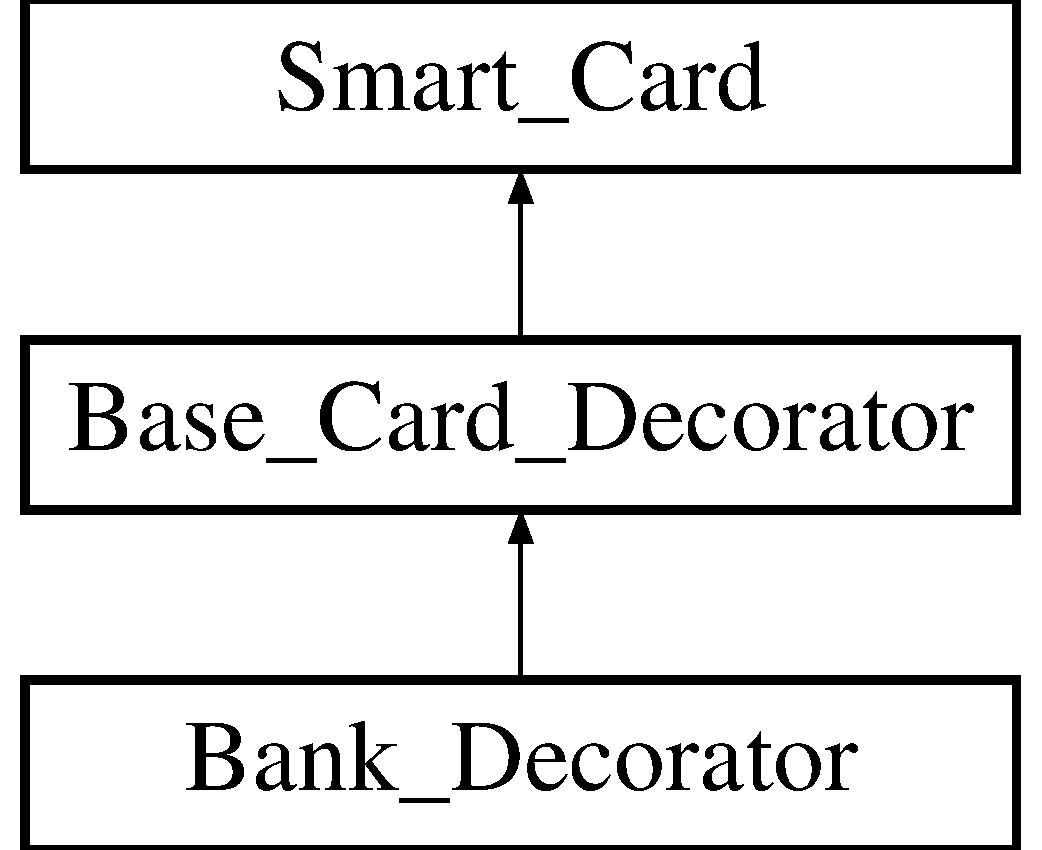
\includegraphics[height=3.000000cm]{classBank__Decorator}
\end{center}
\end{figure}
\subsection*{Public Member Functions}
\begin{DoxyCompactItemize}
\item 
std\+::string \mbox{\hyperlink{classBank__Decorator_a3fe3f99e85f626f1e0a947c630bf7b00}{get\+\_\+bank\+\_\+information}} () override
\begin{DoxyCompactList}\small\item\em Bank information like card number and itn. \end{DoxyCompactList}\item 
\mbox{\Hypertarget{classBank__Decorator_a401bc55d65cce554dd7394d0755fc3d7}\label{classBank__Decorator_a401bc55d65cce554dd7394d0755fc3d7}} 
{\bfseries Bank\+\_\+\+Decorator} (\mbox{\hyperlink{classSmart__Card}{Smart\+\_\+\+Card}} $\ast$s)
\end{DoxyCompactItemize}
\subsection*{Additional Inherited Members}


\subsection{Detailed Description}
All bank information about person. 

\subsection{Member Function Documentation}
\mbox{\Hypertarget{classBank__Decorator_a3fe3f99e85f626f1e0a947c630bf7b00}\label{classBank__Decorator_a3fe3f99e85f626f1e0a947c630bf7b00}} 
\index{Bank\+\_\+\+Decorator@{Bank\+\_\+\+Decorator}!get\+\_\+bank\+\_\+information@{get\+\_\+bank\+\_\+information}}
\index{get\+\_\+bank\+\_\+information@{get\+\_\+bank\+\_\+information}!Bank\+\_\+\+Decorator@{Bank\+\_\+\+Decorator}}
\subsubsection{\texorpdfstring{get\+\_\+bank\+\_\+information()}{get\_bank\_information()}}
{\footnotesize\ttfamily std\+::string Bank\+\_\+\+Decorator\+::get\+\_\+bank\+\_\+information (\begin{DoxyParamCaption}{ }\end{DoxyParamCaption})\hspace{0.3cm}{\ttfamily [inline]}, {\ttfamily [override]}, {\ttfamily [virtual]}}



Bank information like card number and itn. 

\begin{DoxyReturn}{Returns}
Returns card number and individual taxes number 
\end{DoxyReturn}


Reimplemented from \mbox{\hyperlink{classBase__Card__Decorator}{Base\+\_\+\+Card\+\_\+\+Decorator}}.



The documentation for this class was generated from the following file\+:\begin{DoxyCompactItemize}
\item 
Bank\+\_\+\+Decorator.\+h\end{DoxyCompactItemize}

\hypertarget{classBase__Card__Decorator}{}\section{Base\+\_\+\+Card\+\_\+\+Decorator Class Reference}
\label{classBase__Card__Decorator}\index{Base\+\_\+\+Card\+\_\+\+Decorator@{Base\+\_\+\+Card\+\_\+\+Decorator}}


Just simple decorator.  




{\ttfamily \#include $<$base\+\_\+decorator.\+h$>$}

Inheritance diagram for Base\+\_\+\+Card\+\_\+\+Decorator\+:\begin{figure}[H]
\begin{center}
\leavevmode
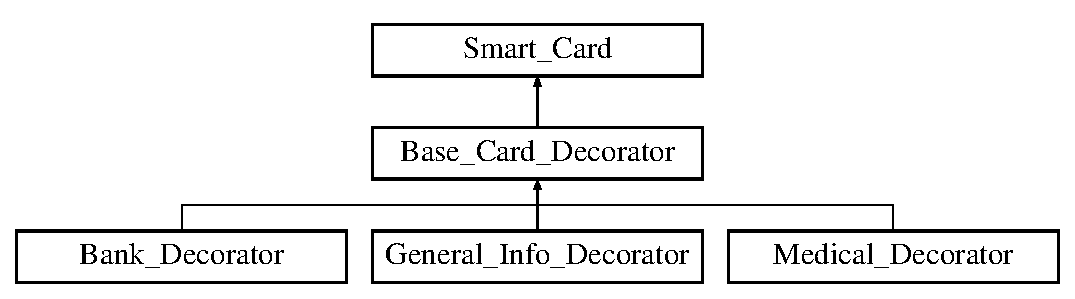
\includegraphics[height=3.000000cm]{classBase__Card__Decorator}
\end{center}
\end{figure}
\subsection*{Public Member Functions}
\begin{DoxyCompactItemize}
\item 
\mbox{\Hypertarget{classBase__Card__Decorator_af25648b0e9cdee9b46f82dbe81e3180f}\label{classBase__Card__Decorator_af25648b0e9cdee9b46f82dbe81e3180f}} 
{\bfseries Base\+\_\+\+Card\+\_\+\+Decorator} (\mbox{\hyperlink{classSmart__Card}{Smart\+\_\+\+Card}} $\ast$s)
\item 
\mbox{\Hypertarget{classBase__Card__Decorator_aa2122fce72c68c372192a548f1cb371c}\label{classBase__Card__Decorator_aa2122fce72c68c372192a548f1cb371c}} 
virtual std\+::string {\bfseries get\+\_\+general\+\_\+information} () override
\item 
\mbox{\Hypertarget{classBase__Card__Decorator_ade292caa83a47707c056fe916fafe4f0}\label{classBase__Card__Decorator_ade292caa83a47707c056fe916fafe4f0}} 
virtual std\+::string {\bfseries get\+\_\+medical\+\_\+information} () override
\item 
\mbox{\Hypertarget{classBase__Card__Decorator_ad93b8c6bc4dcfdd28bdc36c5c133155f}\label{classBase__Card__Decorator_ad93b8c6bc4dcfdd28bdc36c5c133155f}} 
virtual std\+::string {\bfseries get\+\_\+bank\+\_\+information} () override
\end{DoxyCompactItemize}
\subsection*{Public Attributes}
\begin{DoxyCompactItemize}
\item 
\mbox{\Hypertarget{classBase__Card__Decorator_a87669f85c4d5cc25bb0ce63a17b018b2}\label{classBase__Card__Decorator_a87669f85c4d5cc25bb0ce63a17b018b2}} 
\mbox{\hyperlink{classSmart__Card}{Smart\+\_\+\+Card}} $\ast$ {\bfseries wrappee}
\end{DoxyCompactItemize}


\subsection{Detailed Description}
Just simple decorator. 

The documentation for this class was generated from the following file\+:\begin{DoxyCompactItemize}
\item 
base\+\_\+decorator.\+h\end{DoxyCompactItemize}

\hypertarget{classGeneral__Info__Decorator}{}\section{General\+\_\+\+Info\+\_\+\+Decorator Class Reference}
\label{classGeneral__Info__Decorator}\index{General\+\_\+\+Info\+\_\+\+Decorator@{General\+\_\+\+Info\+\_\+\+Decorator}}


Decorator of Info.  




{\ttfamily \#include $<$General\+\_\+\+Info\+\_\+\+Decorator.\+h$>$}

Inheritance diagram for General\+\_\+\+Info\+\_\+\+Decorator\+:\begin{figure}[H]
\begin{center}
\leavevmode
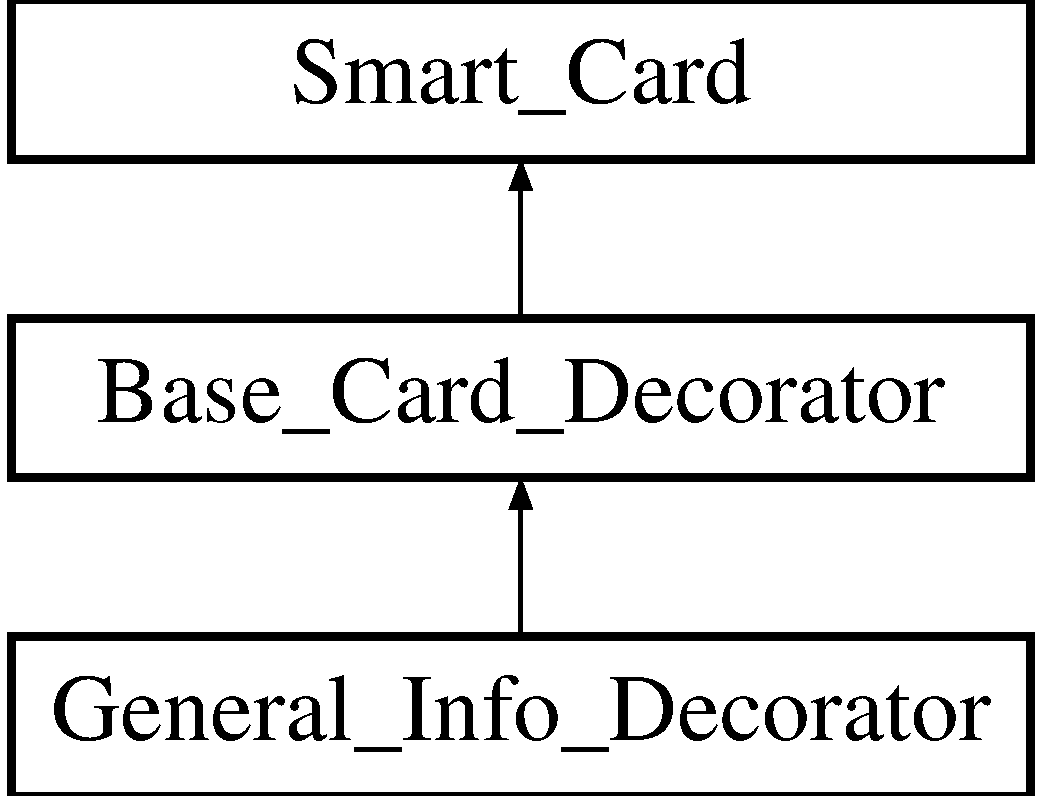
\includegraphics[height=3.000000cm]{classGeneral__Info__Decorator}
\end{center}
\end{figure}
\subsection*{Public Member Functions}
\begin{DoxyCompactItemize}
\item 
std\+::string \mbox{\hyperlink{classGeneral__Info__Decorator_a8bc8c352cf14028a9ef2c3e7dce90db7}{get\+\_\+general\+\_\+information}} () override
\item 
\mbox{\Hypertarget{classGeneral__Info__Decorator_acb5b231e3272f6c97e05969d5725fc94}\label{classGeneral__Info__Decorator_acb5b231e3272f6c97e05969d5725fc94}} 
{\bfseries General\+\_\+\+Info\+\_\+\+Decorator} (\mbox{\hyperlink{classSmart__Card}{Smart\+\_\+\+Card}} $\ast$s)
\end{DoxyCompactItemize}
\subsection*{Additional Inherited Members}


\subsection{Detailed Description}
Decorator of Info. 

\subsection{Member Function Documentation}
\mbox{\Hypertarget{classGeneral__Info__Decorator_a8bc8c352cf14028a9ef2c3e7dce90db7}\label{classGeneral__Info__Decorator_a8bc8c352cf14028a9ef2c3e7dce90db7}} 
\index{General\+\_\+\+Info\+\_\+\+Decorator@{General\+\_\+\+Info\+\_\+\+Decorator}!get\+\_\+general\+\_\+information@{get\+\_\+general\+\_\+information}}
\index{get\+\_\+general\+\_\+information@{get\+\_\+general\+\_\+information}!General\+\_\+\+Info\+\_\+\+Decorator@{General\+\_\+\+Info\+\_\+\+Decorator}}
\subsubsection{\texorpdfstring{get\+\_\+general\+\_\+information()}{get\_general\_information()}}
{\footnotesize\ttfamily std\+::string General\+\_\+\+Info\+\_\+\+Decorator\+::get\+\_\+general\+\_\+information (\begin{DoxyParamCaption}{ }\end{DoxyParamCaption})\hspace{0.3cm}{\ttfamily [inline]}, {\ttfamily [override]}, {\ttfamily [virtual]}}

gives u general information \begin{DoxyReturn}{Returns}
Returns a string from name and date of birth 
\end{DoxyReturn}


Reimplemented from \mbox{\hyperlink{classBase__Card__Decorator}{Base\+\_\+\+Card\+\_\+\+Decorator}}.



The documentation for this class was generated from the following file\+:\begin{DoxyCompactItemize}
\item 
General\+\_\+\+Info\+\_\+\+Decorator.\+h\end{DoxyCompactItemize}

\hypertarget{classMedical__Decorator}{}\section{Medical\+\_\+\+Decorator Class Reference}
\label{classMedical__Decorator}\index{Medical\+\_\+\+Decorator@{Medical\+\_\+\+Decorator}}


Medical life.  




{\ttfamily \#include $<$Medical\+\_\+\+Decorator.\+h$>$}

Inheritance diagram for Medical\+\_\+\+Decorator\+:\begin{figure}[H]
\begin{center}
\leavevmode
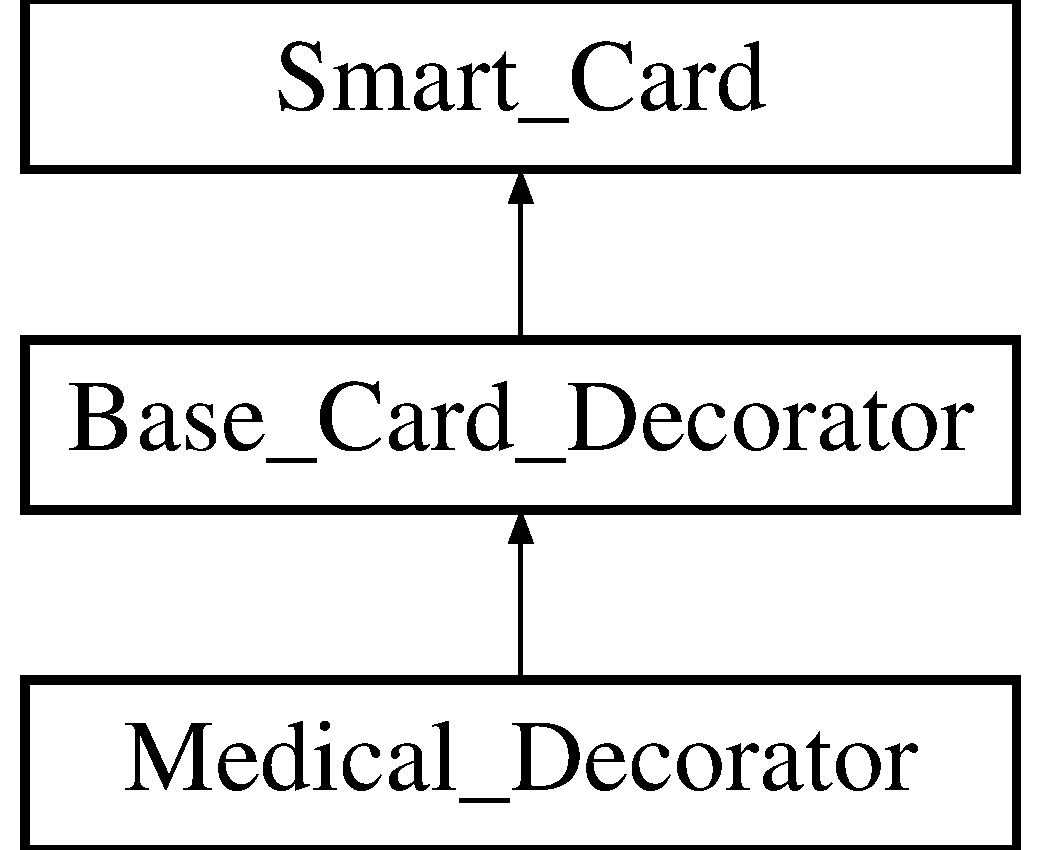
\includegraphics[height=3.000000cm]{classMedical__Decorator}
\end{center}
\end{figure}
\subsection*{Public Member Functions}
\begin{DoxyCompactItemize}
\item 
std\+::string \mbox{\hyperlink{classMedical__Decorator_afde55c4f0f98d5ea566b5a989e631878}{get\+\_\+medical\+\_\+information}} () override
\item 
void \mbox{\hyperlink{classMedical__Decorator_a795110d53121358fcb3d34a187379350}{get\+\_\+blood\+\_\+type}} ()
\item 
\mbox{\Hypertarget{classMedical__Decorator_a57ffdcc3faaca5f05b91aff7b6534d78}\label{classMedical__Decorator_a57ffdcc3faaca5f05b91aff7b6534d78}} 
{\bfseries Medical\+\_\+\+Decorator} (\mbox{\hyperlink{classSmart__Card}{Smart\+\_\+\+Card}} $\ast$s)
\end{DoxyCompactItemize}
\subsection*{Additional Inherited Members}


\subsection{Detailed Description}
Medical life. 

\subsection{Member Function Documentation}
\mbox{\Hypertarget{classMedical__Decorator_a795110d53121358fcb3d34a187379350}\label{classMedical__Decorator_a795110d53121358fcb3d34a187379350}} 
\index{Medical\+\_\+\+Decorator@{Medical\+\_\+\+Decorator}!get\+\_\+blood\+\_\+type@{get\+\_\+blood\+\_\+type}}
\index{get\+\_\+blood\+\_\+type@{get\+\_\+blood\+\_\+type}!Medical\+\_\+\+Decorator@{Medical\+\_\+\+Decorator}}
\subsubsection{\texorpdfstring{get\+\_\+blood\+\_\+type()}{get\_blood\_type()}}
{\footnotesize\ttfamily void Medical\+\_\+\+Decorator\+::get\+\_\+blood\+\_\+type (\begin{DoxyParamCaption}{ }\end{DoxyParamCaption})\hspace{0.3cm}{\ttfamily [inline]}}

brief Gets blood type from base \mbox{\Hypertarget{classMedical__Decorator_afde55c4f0f98d5ea566b5a989e631878}\label{classMedical__Decorator_afde55c4f0f98d5ea566b5a989e631878}} 
\index{Medical\+\_\+\+Decorator@{Medical\+\_\+\+Decorator}!get\+\_\+medical\+\_\+information@{get\+\_\+medical\+\_\+information}}
\index{get\+\_\+medical\+\_\+information@{get\+\_\+medical\+\_\+information}!Medical\+\_\+\+Decorator@{Medical\+\_\+\+Decorator}}
\subsubsection{\texorpdfstring{get\+\_\+medical\+\_\+information()}{get\_medical\_information()}}
{\footnotesize\ttfamily std\+::string Medical\+\_\+\+Decorator\+::get\+\_\+medical\+\_\+information (\begin{DoxyParamCaption}{ }\end{DoxyParamCaption})\hspace{0.3cm}{\ttfamily [inline]}, {\ttfamily [override]}, {\ttfamily [virtual]}}

Medical info \begin{DoxyReturn}{Returns}
Blood type and insurance 
\end{DoxyReturn}


Reimplemented from \mbox{\hyperlink{classBase__Card__Decorator}{Base\+\_\+\+Card\+\_\+\+Decorator}}.



The documentation for this class was generated from the following file\+:\begin{DoxyCompactItemize}
\item 
Medical\+\_\+\+Decorator.\+h\end{DoxyCompactItemize}

\hypertarget{classSmart__Card}{}\section{Smart\+\_\+\+Card Class Reference}
\label{classSmart__Card}\index{Smart\+\_\+\+Card@{Smart\+\_\+\+Card}}
Inheritance diagram for Smart\+\_\+\+Card\+:\begin{figure}[H]
\begin{center}
\leavevmode
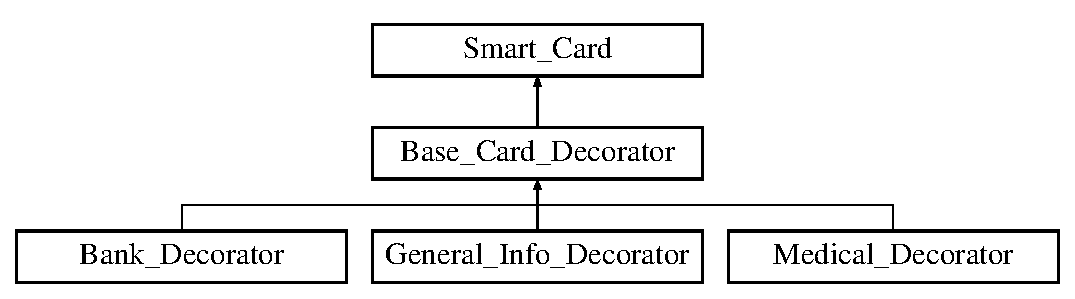
\includegraphics[height=3.000000cm]{classSmart__Card}
\end{center}
\end{figure}
\subsection*{Public Member Functions}
\begin{DoxyCompactItemize}
\item 
\mbox{\Hypertarget{classSmart__Card_a4f4fe2f699499066a4d4dfac2b4a1d8d}\label{classSmart__Card_a4f4fe2f699499066a4d4dfac2b4a1d8d}} 
{\bfseries Smart\+\_\+\+Card} (int \+\_\+id=0)
\item 
\mbox{\Hypertarget{classSmart__Card_a05e1d5bc72008ee610e7f41ca33ce1f6}\label{classSmart__Card_a05e1d5bc72008ee610e7f41ca33ce1f6}} 
const std\+::string {\bfseries get\+\_\+name} ()
\item 
\mbox{\Hypertarget{classSmart__Card_a595d127eba331f581be4123d875f5d66}\label{classSmart__Card_a595d127eba331f581be4123d875f5d66}} 
const std\+::string {\bfseries get\+\_\+date\+\_\+of\+\_\+birth} ()
\item 
\mbox{\Hypertarget{classSmart__Card_aaf70c68d37bfbe00d46ccc88ca19892c}\label{classSmart__Card_aaf70c68d37bfbe00d46ccc88ca19892c}} 
const std\+::string {\bfseries get\+\_\+taxes\+\_\+number} ()
\item 
\mbox{\Hypertarget{classSmart__Card_a784debae8edda24f37544f7194b04fcc}\label{classSmart__Card_a784debae8edda24f37544f7194b04fcc}} 
const std\+::string {\bfseries get\+\_\+insurance} ()
\item 
\mbox{\Hypertarget{classSmart__Card_a7fd85140ca3d67319e91023367db018e}\label{classSmart__Card_a7fd85140ca3d67319e91023367db018e}} 
const std\+::string {\bfseries get\+\_\+bank\+\_\+card\+\_\+number} ()
\item 
\mbox{\Hypertarget{classSmart__Card_a820d631da800e09e3990829c3dd30a2b}\label{classSmart__Card_a820d631da800e09e3990829c3dd30a2b}} 
const std\+::string {\bfseries get\+\_\+driving\+\_\+licence} ()
\item 
\mbox{\Hypertarget{classSmart__Card_a4e5bbbf29e25e9657940f4091f3e1ba0}\label{classSmart__Card_a4e5bbbf29e25e9657940f4091f3e1ba0}} 
virtual std\+::string {\bfseries get\+\_\+general\+\_\+information} ()
\item 
\mbox{\Hypertarget{classSmart__Card_a9dfaf07cce3ea7ae2d5d159d60727fed}\label{classSmart__Card_a9dfaf07cce3ea7ae2d5d159d60727fed}} 
virtual std\+::string {\bfseries get\+\_\+medical\+\_\+information} ()
\item 
\mbox{\Hypertarget{classSmart__Card_a1a13e7a3363ca29311b46c7112ef3982}\label{classSmart__Card_a1a13e7a3363ca29311b46c7112ef3982}} 
virtual std\+::string {\bfseries get\+\_\+bank\+\_\+information} ()
\end{DoxyCompactItemize}


The documentation for this class was generated from the following file\+:\begin{DoxyCompactItemize}
\item 
Smart\+\_\+\+Card.\+h\end{DoxyCompactItemize}

%--- End generated contents ---

% Index
\backmatter
\newpage
\phantomsection
\clearemptydoublepage
\addcontentsline{toc}{chapter}{Index}
\printindex

\end{document}
